\section{Optische Grössen}

\subsection{Licht}

Licht kann auf mehrere Arten beschrieben werden:


\subsubsection{Lichtstrahlen}

\begin{minipage}[t]{0.48\columnwidth}
    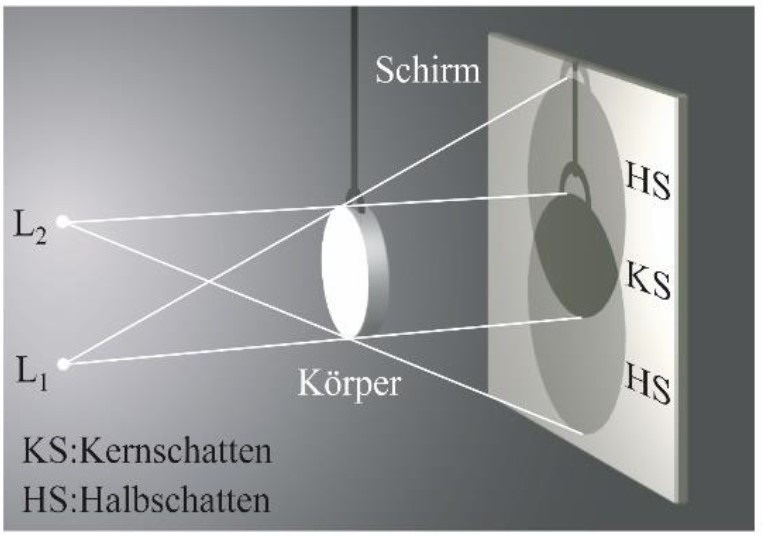
\includegraphics[width=\columnwidth, align=t]{images/lichtstrahlen.jpg}
\end{minipage}
\hfill
\begin{minipage}[t]{0.48\columnwidth}
    Die \textbf{geometrische Optik} oder \textbf{Strahlenoptik} geht davon aus, dass sich das Licht im Vakuum als \textbf{geradliniger Strahl} ausbreitet.

    \medskip

    Mit der geometrischen Optik können die Phänomene Reflexion und Brechung erklärt werden.
\end{minipage}


\subsubsection{Lichtwellen}

\begin{minipage}[t]{0.48\columnwidth}
    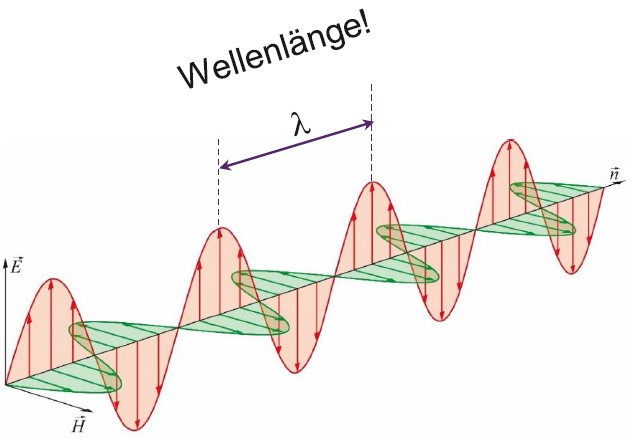
\includegraphics[width=\columnwidth, align=t]{images/lichtwelle.jpg}
\end{minipage}
\hfill
\begin{minipage}[t]{0.48\columnwidth}
    Licht wird als elektromagnetische Welle modelliert.

    \medskip
    
    Bild: linear polarisierte Welle
\end{minipage}


\medskip

\para{Lichtfarben und ihre Frequenzen / Wellenlängen} 

\begin{minipage}[c]{0.42\columnwidth}
    \begin{ctabular}{l c}
        \toprule
        \textbf{Farbe}                          & \textbf{Wellenlänge in $\bm{\nano\meter}$}    \\
        \midrule
        \color{red!50!blue!80!white}violett     & 380 \ldots 435                                \\
        \midrule
        \color{blue}blau                        & 435 \ldots 465                                \\
        \midrule
        \color[HTML]{35c2bd}blaugrün            & 465 \ldots 485                                \\
        \midrule
        \color{green!80!black}grün              & 485 \ldots 565                                \\
        \midrule
        \color{yellow!75!red}gelb               & 565 \ldots 590                                \\
        \midrule
        \color{orange}orange                    & 590 \ldots 630                                \\
        \midrule
        \color{red}rot                          & 630 \ldots 780                                \\
        \bottomrule
    \end{ctabular}
\end{minipage}
\hfill
\begin{minipage}[c]{0.55\columnwidth}
    $$ \boxed{ \lambda = \frac{c}{f} }  \qquad \qquad \qquad \boxed{ \frac{\Delta f}{\Delta \lambda} = \frac{c}{\lambda^2}} $$

    \begin{tabular}{c l c}
        $\lambda$   & Wellenlänge                                       & $[\lambda] = \meter$                          \\
        $c$         & Lichtgeschwindigkeit                              & $[c] = \frac{\meter}{\second}$                \\
                    & $c = 300 \cdot 10^6 \, \frac{\meter}{\second}$    &                                               \\
        $f$         & Frequenz                                          & $[f] = \mathrm{\frac{1}{\second} = \hertz}$ 
    \end{tabular}
\end{minipage}


\subsubsection{Lichtteilchen}

Modellvorstellung des Lichts als ein Fluss von Lichtteilchen (\textbf{Photonen})


$$ \boxed{ E = h \cdot f } $$

\begin{tabular}{c l c}
	$E$ & Energie \textbf{eines} Photons & $[E] = \joule$ \\
	$h$ & Planck'sche Konstante $6.626 \cdot 10^{-34} \frac{\joule}{\hertz}$ & $[h] = \frac{\joule}{\hertz}$ \\
	$f$ & Frequenz & $[f] = \mathrm{\frac{1}{\second} = \hertz}$
\end{tabular}


\subsection{Lichtquellen}

\subsubsection{Thermische Strahler}

\textbf{Schwarzkörper-Modell}: Modell eines Körpers, der in alle Richtungen abstrahlt (und energetisch im Gleichgewicht ist) \\
Ein Schwarzkörper strahlt \textbf{alle} Lichtfarben ab. (auch die für den Mensch nicht sichtbaren.) 

\medskip


\begin{minipage}[t]{0.52\columnwidth}
    \para{Glühbirnen}

    Muss auf allen Wellenlängen angeregt werden, um schliesslich sichtbares Licht abzustrahlen. \\
    \textrightarrow\ Es wird viel Energie nicht nutzbar 'verheizt'
\end{minipage}
\hfill
\begin{minipage}[t]{0.44\columnwidth}
    \para{LEDs}

    Können mit einer bestimmten Frequenz angeregt werden und strahlen nur gewünschtes Licht ab.
    \textrightarrow\ energieeffizient
\end{minipage}



\subsubsection{Lumineszenz}

\begin{minipage}[t]{0.3\columnwidth}
    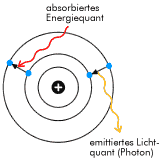
\includegraphics[width=\columnwidth, align=t]{images/lumineszenz.png}
\end{minipage}
\hfill
\begin{minipage}[t]{0.65\columnwidth}
    \begin{itemize}
        \item Elektronen werden angeregt und steigen in energetisch höheren Zustand.
        \item Sobald die Elektronen wieder in ihren Grundzustand zurückkehren wird ein Lichtquant (Photon) abgestrahlt.
        \item Die Leuchtfarbe wird durch die Frequenz der Anregung bestimmt.
    \end{itemize}

    \medskip
    \begin{description}
        \item[Fluoreszenz:] kein Nachleuchten
        \item[Phosphoreszenz:] mit Nachleuchten
    \end{description}
\end{minipage}


\subsection{Messgrössen}

\subsubsection{Radiometrie}

Physikalische Messgrössen der elekromagnetischen Strahlung


\subsubsection{Photometrie}

Radiometrische Grössen, gewichtet mit dem photometrischen Strahlungsäquivalent $K$, welches die \textbf{Empfindlichkeit des menschlichen Auges} angibt.


\paragraph{Photometrischen Strahlungsäquivalent $\bm{K}$}

Gibt die Empfindlichkeit des menschlichen Auges wieder und ist eine empirisch genormte Kurve \\
\textrightarrow\ Menschliches Auge ist bei Wellenlänge von $555 \, \nano\meter$  (grüne Farbe) am empfindlichsten \\
\textrightarrow\ Entspricht $638 \, \frac{\lumen}{\watt}$


\subsection{Gegenüberstellung: Radiometrie -- Photometrie}

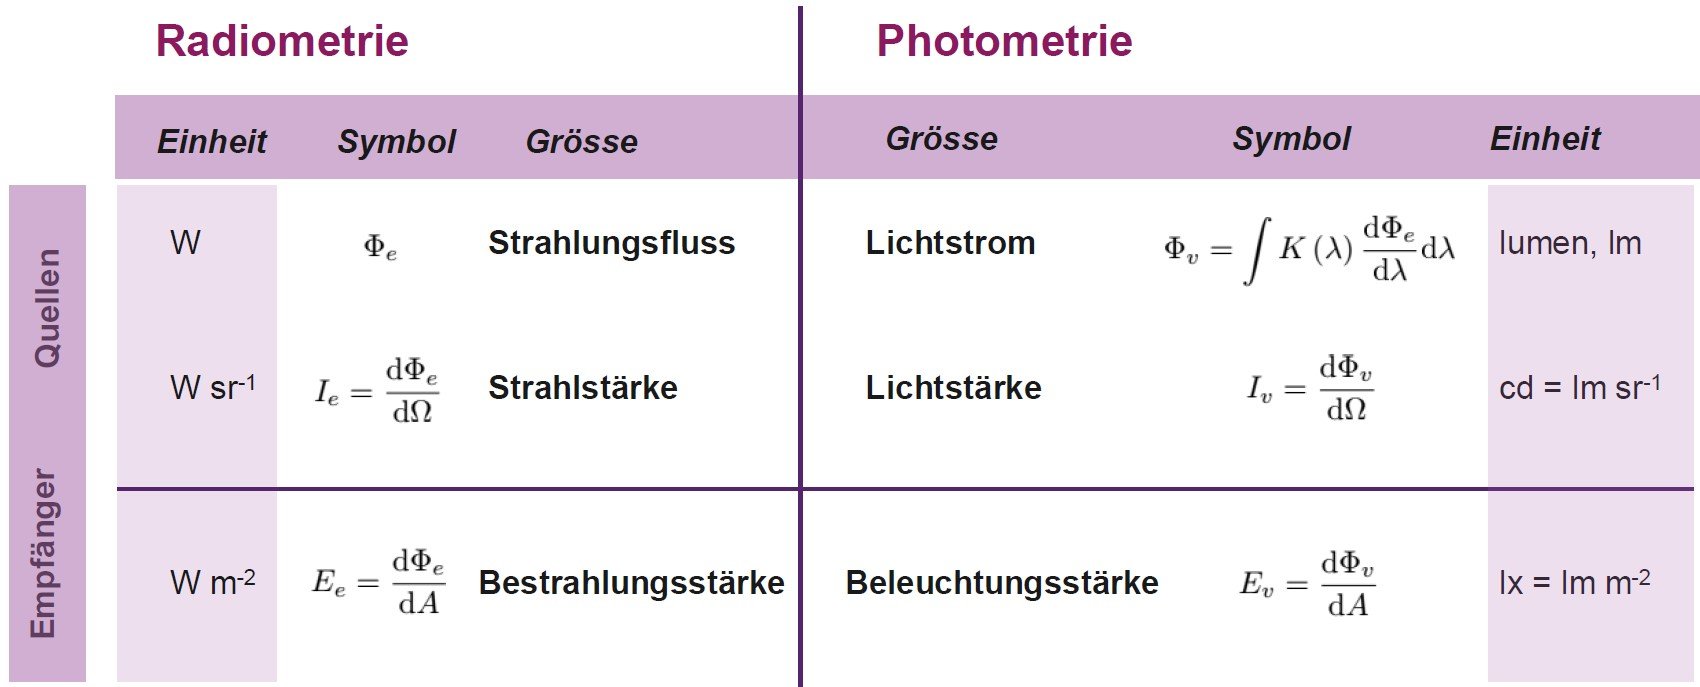
\includegraphics[width=\columnwidth]{images/radiometrie_photometrie.jpg}


\subsection{Raumwinkel}

\subsubsection{Winkel in der Ebene}

\begin{minipage}[t]{0.35\columnwidth}
    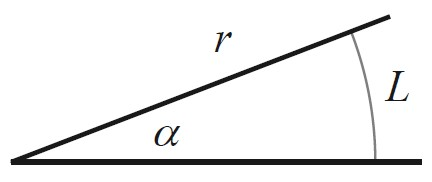
\includegraphics[width=\columnwidth, align=t]{images/winkel_ebene.jpg}
\end{minipage}
\hfill
\begin{minipage}[t]{0.6\columnwidth}
    Länge des Bogens auf einem Kreis mit $r = 1 \, \meter$ 

    \medskip

    \begin{minipage}[c]{0.48\columnwidth}
        $$ \boxed{ \alpha = \frac{L}{r}  } $$ 
    \end{minipage}
    \hfill
    \begin{minipage}[c]{0.48\columnwidth}
        Vollkreis: $2 \, \pi$\\
        $[\alpha] = \rad$ 
    \end{minipage}
\end{minipage}


\subsubsection{Winkel im Raum}

\begin{minipage}[t]{0.3\columnwidth}
    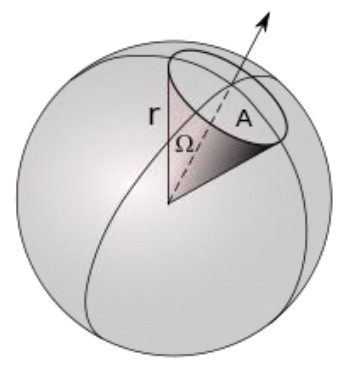
\includegraphics[width=\columnwidth, align=t]{images/winkel_raum.jpg}
\end{minipage}
\hfill
\begin{minipage}[t]{0.66\columnwidth}
    Aufgespannte Fläche, projiziert auf eine Kugel mit $r = 1 \, \meter$
    
    \medskip

    \begin{minipage}[c]{0.48\columnwidth}
        $$ \boxed{ \Omega = \frac{A}{r^2} = \frac{A}{1 \, \meter\squared} } $$
    \end{minipage}
    \hfill
    \begin{minipage}[c]{0.48\columnwidth}
        Kugel: $4 \, \pi$ \\
        $[\Omega] = \steradian$ (Steradiant) 
    \end{minipage}
\end{minipage}

